$(p,q)$-horse is a generalisation of chess Knight who moves $p$ steps one
axis and $q$ steps another (perpendicular) axis. Ordinary chess
Knight is thus a $(2,1)$-horse.

Your task is to determine how many moves $(p,q)$-horse needs to go from one
cell on $M$x$N$ chess-board to another.

\begin{figure}[h!]
    \centering
    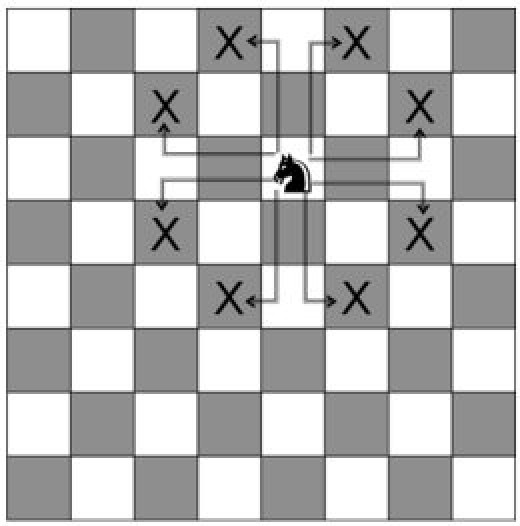
\includegraphics[scale=0.25]{pq.jpg}
    \caption{All possible $(2,1)$-horse moves}
\end{figure}

\subsection*{Input}

Each test case is a single line containing 8 integers $M$, $N$, $p$, $q$,
     $x_1$, $y_1$, $x_2$, $y_2$
     $(1 \le x_1, x_2 \le M, 1 \le y_1, y_2 \le N, 0 \le p \le M \le 1000, 0
         \le q \le N \le 1000)$.

\subsection*{Output}
For each test case, output a line with the integer $k$, the minimum number of
moves required by the $(p,q)$-horse to go from $(x_1,y_1)$ to $(x_2,y_2)$.

If it is impossible for the $(p,q)$-horse to go from $(x_1,y_1)$ to
$(x_2,y_2)$, then print a line containing -1 instead.


\begin{table}[!h]
\centering
\begin{tabular}{|l|l|}
\hline
\begin{minipage}[t]{3in}
\textbf{Sample Input}
\begin{verbatim}
3 3 1 1 1 1 3 3
2 2 1 1 1 1 1 2
\end{verbatim}
\vspace{1mm}
\end{minipage}
&

\begin{minipage}[t]{3in}
\textbf{Sample Output}
\begin{verbatim}
2
-1
\end{verbatim}
\vspace{1mm}
\end{minipage} \\
\hline
\end{tabular}
\end{table}

\newpage
